%%%%%%%%%%%%%%%%%%%%%%%%%%%%%%%%%%%%%%%%%
% The Legrand Orange Book
% LaTeX Template
% Version 2.1.1 (14/2/16)
%
% This template has been downloaded from:
% http://www.LaTeXTemplates.com
%
% Original author:
% Mathias Legrand (legrand.mathias@gmail.com) with modifications by:
% Vel (vel@latextemplates.com)
%
% License:
% CC BY-NC-SA 3.0 (http://creativecommons.org/licenses/by-nc-sa/3.0/)
%
% Compiling this template:
% This template uses biber for its bibliography and makeindex for its index.
% When you first open the template, compile it from the command line with the 
% commands below to make sure your LaTeX distribution is configured correctly:
%
% 1) pdflatex main
% 2) makeindex main.idx -s StyleInd.ist
% 3) biber main
% 4) pdflatex main x 2
%
% After this, when you wish to update the bibliography/index use the appropriate
% command above and make sure to compile with pdflatex several times 
% afterwards to propagate your changes to the document.
%
% This template also uses a number of packages which may need to be
% updated to the newest versions for the template to compile. It is strongly
% recommended you update your LaTeX distribution if you have any
% compilation errors.
%
% Important note:
% Chapter heading images should have a 2:1 width:height ratio,
% e.g. 920px width and 460px height.
%
%%%%%%%%%%%%%%%%%%%%%%%%%%%%%%%%%%%%%%%%%

%----------------------------------------------------------------------------------------
%	PACKAGES AND OTHER DOCUMENT CONFIGURATIONS
%----------------------------------------------------------------------------------------

\documentclass[11pt,fleqn]{book} % Default font size and left-justified equations

\usepackage{ifthen} 
\newboolean{VersionProf}
\setboolean{VersionProf}{false}

\usepackage{wasysym}
\usepackage{esint} % various fancy integral symbols
\usepackage{tikz}
\usepackage{tikz-3dplot}
\usepackage{pgfplots}
\pgfplotsset{compat=1.17}
\usetikzlibrary{patterns}
\usepackage{tkz-euclide} 
\usepackage{mathtools}
\usepackage{xurl}
\usepackage[version=4,arrows=pgf-filled,
textfontname=sffamily,
mathfontname=mathsf]{mhchem}
\usepackage{gensymb}
\usepackage{tabularray}
\usepackage{csquotes}

\usepackage[french]{babel}
\usepackage{dingbat}

\usepackage{environ}
\usepackage{wrapfig}

\NewEnviron{solution}{%
    \ifthenelse{\boolean{VersionProf}}{\begin{solutionA}
        \BODY%*
        \end{solutionA}
    }{%
        \relax%
    }%
}%

\usetikzlibrary {arrows.meta} 

\newcommand{\degC}{{\degree}C}
\newcommand{\dd}{\mathrm{d}}
\newcommand{\div}{\mathrm{div}}
\newcommand{\rot}{\vv{\mathrm{div}}}
\newcommand{\grad}{\vv{\mathrm{grad}}}

\tikzset{
    support/.style={
        pattern=north east lines,
        draw=none,
        minimum width=0.3,
        minimum height=0.6
    }
    ,>=latex
}

\usepackage[d]{esvect}

%SPECIFIC TO THIS CHAPTER
\usepackage{physics}
\usepackage{ifthen}
\usepackage[outline]{contour} % glow around text
\usetikzlibrary{calc} % for pic
\usetikzlibrary{angles,quotes} % for pic
\usetikzlibrary{patterns}
\tikzset{>=latex} % for LaTeX arrow head
\contourlength{1.2pt}

\colorlet{myred}{red!65!black}
\definecolor{myred}{RGB}{127,0,255}
\tikzstyle{ground}=[preaction={fill,top color=black!10,bottom color=black!5,shading angle=20},
                    fill,pattern=north east lines,draw=none,minimum width=0.3,minimum height=0.6]
\tikzstyle{mass}=[line width=0.6,myred,fill=myred!40,rounded corners=1,
                  top color=myred!40,bottom color=myred!20,shading angle=20]
\tikzstyle{rope}=[myred!30,line width=1.2,line cap=round] %very thick

% FORCES SWITCH
\tikzstyle{force}=[->,myred,ultra thick,line cap=round]
\tikzstyle{Fproj}=[force,myred!60]
\newboolean{showforces}
\setboolean{showforces}{true}
%----------------------------------------------------------------------------------------

\input{structure} % Insert the commands.tex file which contains the majority of the structure behind the template

\begin{document}

%----------------------------------------------------------------------------------------
%	TABLE OF CONTENTS
%----------------------------------------------------------------------------------------

%\usechapterimagefalse % If you don't want to include a chapter image, use this to toggle images off - it can be enabled later with \usechapterimagetrue

\chapterimage{filmB.jpg} % Table of contents heading image

%\pagestyle{empty} % No headers

%\tableofcontents % Print the table of contents itself

%\cleardoublepage % Forces the first chapter to start on an odd page so it's on the right

%\pagestyle{fancy} % Print headers again



%\part{\'{E}lectromagnétisme}

\setcounter{chapter}{13}

\chapter{Conversion électrochimique d'énergie}

Dans les premiers chapitres d'électrochimie, nous avons montré comment le caractère spontané d'une réaction chimique peut être exploité pour extraire de l'énergie, notamment sous forme thermique (dans le cas des réactions exothermiques) : c'est ce qui est exploité dans tous les appareils à combustion, tels que le moteur thermique d'une voiture, les réacteurs d'un avion, une cuisinière... Ce type de processus se retrouve également dans la nature, par exemple dans les réactions de fusion nucléaire exothermiques se produisant dans les étoiles.

Nous allons désormais nous intéresser à une autre forme d'énergie : l'énergie électrique. Dans le cas des réactions d'oxydoréduction, des échanges d'électrons interviennent de manière spontanée et il est possible d'exploiter cette propriété pour produire de l'énergie électrique à partir d'une réaction chimique. Par ailleurs, nous verrons que ce processus a l'avantage d'être (partiellement) réversible : il est possible de forcer une réaction chimique non spontanée en fournissant de l'énergie électrique.

Dans ce premier chapitre, nous nous intéresserons ainsi aux aspects thermodynamiques des réactions d'oxydoréduction et à leurs applications en termes de stockage et de conversion d'énergie électrique. Dans un second chapitre, nous verrons les aspects cinétiques de la conversion électrique d'énergie et en particulier les limites que la cinétique peut apporter à ce processus.

\section{Fonctionnement d'une pile}

\subsection{Rappels : anode, cathode, équation bilan}

\begin{figure}[htbp]
	\centering 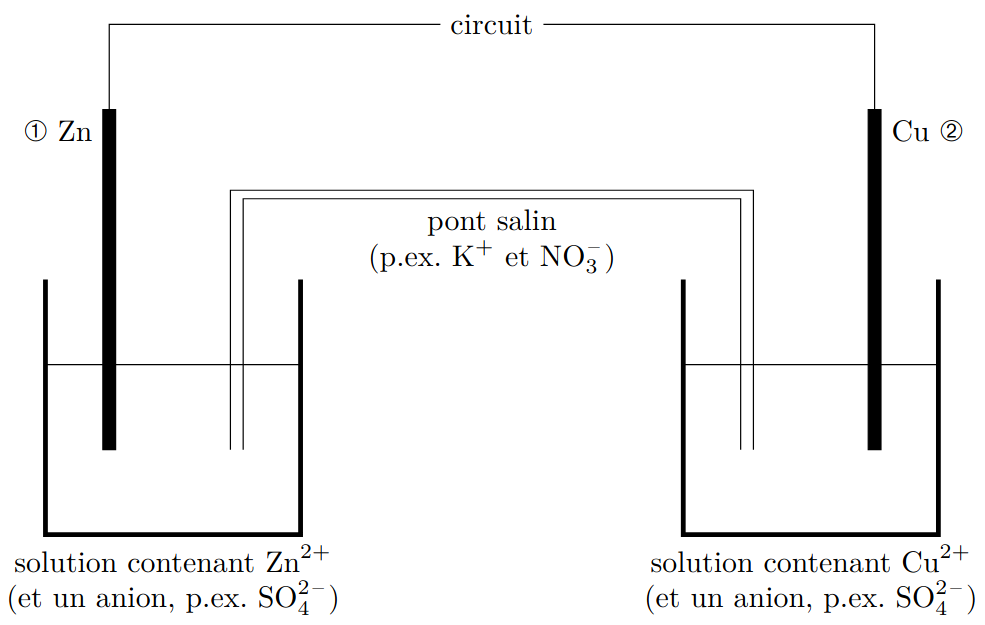
\includegraphics[width=0.8\linewidth]{pile_daniell.png}
	\caption{Schéma de la pile Daniell. Source : poly de cours de Etienne Thibierge.}
\end{figure}

Considérons la pile Daniell, l'une des piles les plus simples qui puissent être construites : elle fait intervenir les deux couples d'oxydoréduction $\ce{Fe^{2+}(aq)/Fe(s)}$ et $\ce{Cu^{2+}/Cu(s)}$. Nous définissons les deux électrodes par la nature de la demi-réaction qui s'y produit :
\begin{definition}
	L'anode est une électrode sur laquelle se produit une oxydation. La cathode est l'électrode sur laquelle se produit une réduction.
\end{definition}


Dans la pile Daniell, on a une oxydation à l'anode qui est l'électrode de zinc : 
\begin{equation}
	\ce{Zn(s) \rightarrow Zn^{2+}(aq) + 2 e^-}
\end{equation}
et on a une réduction à la cathode qui est l'électrode de cuivre :
\begin{equation}
	\ce{Cu^{2+}(aq) + 2 e^- \rightarrow Cu(s)}
\end{equation}
On obtient alors l'équation bilan de la pile :
\begin{equation}
	\ce{Cu^{2+}(aq) + Zn(s) = Cu(s) + Zn^{2+}(aq)}
\end{equation}

Le dispositif de la pile, en séparant physiquement les deux réactifs, permet de canaliser les électrons à travers un circuit électrique extérieur et ainsi de récupérer de l'énergie électrique à partir de la réaction chimique.


\subsection{Bilan électrique d'une pile ou d'un électrolyseur}

La pile Daniell est un exemple d'une catégorie plus large de systèmes correspondant aux piles électrochimiques, utilisées pour convertir de l'énergie chimique en énergie électrique : une réaction chimique se fait spontanément et libère une énergie $-W_e >0$ qui peut être utilisée pour alimenter un appareil électrique. L'énergie totale pouvant être utilisée est limitée par la variation d'enthalpie libre $\Delta G$ comme nous l'avons déjà vu. Mais nous pouvons également faire un bilan électrique :
\begin{capex}
	A partir de l'exemple de la pile Daniell, établir la charge maximale $q_{\rm max}$ qui peut être débitée par la pile en fonction du volume $V_0$ des solutions et de la concentration initiale $c_0$ en ions $\ce{Cu^{2+}}$ et $\ce{Zn^{2+}}$. 
\end{capex}

Il est également possible de réaliser le procédé inverse : il s'agit de l'électrolyse. Une réaction chimique non spontanée est forcée en imposant une différence de potentiel entre deux électrodes suffisante pour que la réaction chimique puisse se faire spontanément. C'est le cas, par exemple, de l'électrolyse de l'eau qui sert à former le dihydrogène :
\begin{equation}
	\ce{2 H2O(l) = 2 H2(g) + O2 (g)}
\end{equation}

\begin{remark}
	Cette réaction est une réaction dite de \textbf{dismutation} : l'eau réagit comme oxydant d'un premier couple $\ce{H2O / H2}$ et réducteur d'un second couple $\ce{O2 / H2O}$ pour former ces deux espèces chimiques.
	
	La réaction opposée est appelée réaction de \textbf{médiamutation}.
\end{remark}

\begin{capex}
	A l'aide d'un bilan de quantité de matière, relier la durée $\Delta t$ de l'électrolyse au courant imposé pour réaliser l'électrolyse, noté $i$, et à la masse de dihydrogène produite par électrolyse $m_{\ce{H2}}$.
\end{capex}

\subsection{Bilan énergétique}

Nous avons vu dans le cours de thermochimie que pour un système thermodynamique en évolution monotherme et monobare, l'enthalpie libre $G$ ne peut que diminuer. Nous allons établir une propriété similaire dans le cadre d'un système qui peut échanger du travail électrique $W_e$ avec l'extérieur. Au cours d'un intervalle de temps $\dd t$, l'énergie électrique cédée par la pile au dipôle électrique est donnée par :
\begin{equation}
	-\delta W_e = E i \dd t = E \dd q
\end{equation}
où $q$ est la charge échangée dans le sens du courant ($i = \dd q / \dd t$) et $E$ est la force électromotrice de la pile (tension aux bornes de la pile en convention générateur, et aux bornes du dipôle en convention récepteur).

\begin{capex}
	Etablir une inégalité reliant l'énergie électrique fournie par la pile $-W_e$ à la variation d'enthalpie dans la pile $\Delta G$. En déduire que l'énergie totale que l'on peut extraire de la pile est limitée.
\end{capex}

Considérons maintenant une transformation quelconque infinitésimale, nous savons qu'au cours de cette transformation, la variation d'enthalpie libre dans la pile est donnée par :
\begin{equation}
	\dd G = \Delta_r G \dd \xi
\end{equation}
Par ailleurs, nous savons également que nous pouvons calculer la variation d'enthalpie libre sur un chemin réversible :
\begin{align}
	\dd G &= \dd (U + PV - TS) \\
	&= \dd U + P \dd V - T \dd S \quad \mathrm{(monotherme et monobare)} \\
	&= \delta W_{\rm pression} + \delta W_{\rm elec} + \delta Q_{\rm rev} + P \dd V - T \dd S \\
	&= \delta W_{\elec} \\
	&= -E \dd q
\end{align}
car $\delta Q_{\rm rev} = T \dd S$ et $\delta W_{\rm pression} = - P \dd V$.

\begin{capex}
	Relier le transfert de charge $\dd q$ dans la pile à l'avancement $\dd \xi$ de la réaction d'oxydoréduction. En déduire une relation entre l'enthalpie libre de réaction $\Delta_r G$ et la différence de potentiel aux bornes de la pile. Que vaut la différence de potentiel à l'équilibre thermodynamique ?
\end{capex}

On définit ainsi le Faraday, charge d'une mole d'électrons en valeur absolue :
\begin{definition}{Faraday}
	Le Faraday est l'opposé de la charge d'une mole d'électrons :
	\begin{equation}
		\mathcal{F} = \mathcal{N}_A e = 96\,500\,\mathrm{C}\cdot\mathrm{mol}^{-1}
	\end{equation}
\end{definition}

Nous pouvons alors réinjecter dans cette relation l'expression de l'enthalpie libre de réaction que nous avons vue en thermochimie :
\begin{equation}
	\Delta_r G = \sum_i \nu_i \mu_i = \sum_i \nu_i \left( \mu_i^\circ(T) + R T \ln(a_i) \right)
\end{equation}
En combinant avec la loi précédente, nous obtenons alors :
\begin{equation}
	E = E_{+} - E_{-} = \frac{1}{n \mathcal{F}} \left( \mu_i^\circ(T) + R T \ln(a_i) \right)
\end{equation}
Nous pouvons remarquer que, a priori, le potentiel de la cathode ne dépend que des propriétés des constituants de la cathode, et pareillement pour l'anode. Ainsi nous pouvons identifier les termes correspondant à $E_{+}$ et $E_{-}$ dans l'équation et nous obtenons :
\begin{align}
	E_{\rm cathode} &= E^\circ(\ce{Cu^{2+}/Cu}) + \frac{R T}{n \mathcal{F}} \ln \left( \frac{a(\ce{Cu^{2+}})}{a(\ce{Cu})}  \right)\\
	E_{\rm anode} &= E^\circ(\ce{Zn^{2+}/Zn}) + \frac{R T}{n \mathcal{F}} \ln \left( \frac{a(\ce{Zn^{2+}})}{a(\ce{Zn})}  \right)
\end{align}
\begin{remark}
	Il pourrait être tentant de définir $E^\circ(\ce{Cu^{2+}/Cu}) = \dfrac{\mu^\circ(\ce{Cu^{2+}})-\mu^\circ(\ce{Cu^{2+}})}{n \mathcal{F}}$, mais en réalité les potentiels de référence sont définis à une constante près puisque seule la différence de potentiel apparaît dans l'équation finale. On prend pour référence le potentiel standard du couple $\ce{H+/H2}$ :
	\begin{equation}
		E^\circ(H+/H2) = 0\,\mathrm{V}
	\end{equation}
\end{remark}

Nous avons ici démontré (pour un cas particulier) la loi de Nernst que vous avez vue en MPSI :
\begin{theorem}[Formule de Nernst]
	Soit un couple d'oxydant réducteur $Ox/Red$ associé à la demi-équation électronique $\alpha Ox + n \ce{e}^- = \beta Red$. Alors, le potentiel d'une solution où coexistent l'oxydant et le réducteur est donné par :
	\begin{align}
		E &= E^\circ(Ox/Red) + \frac{R T}{n \mathcal{F}} \ln \left( \frac{a(Ox)^\alpha}{a(Red)^\beta} \right) \\
		&= E^\circ(Ox/Red) + \frac{0.06}{n} \log \left( \frac{a(Ox)^\alpha}{a(Red)^\beta} \right)
	\end{align}
	où on a fait l'application numérique $R T/\mathcal{F} \times  \ln 10 \approx 0.06$\,V.
\end{theorem}

\textbf{Attention !} Dans le cas où la demi-équation électronique fait intervenir d'autres espèces (par exemple de l'eau, des ions hydrohyde ou oxonium) il convient de toujours équilibrer la demi-équation électronique avec des protons $\ce{H^+}$. En effet, le potentiel dépend du pH de la solution et les potentiels standard sont par convention tabulés à $pH = 0$ (il est ensuite possible de calculer le potentiel standard pour d'autres valeurs de pH à partir de la formule de Nernst). On peut alors utiliser la formule de Nernst en prenant soin d'inclure l'activité des protons à l'intérieur du logarithme, comme pour un quotient réactionnel.

\subsection{Lien entre potentiel et constante de réaction}

\begin{capex}
	A partir de la formule de Nernst, retrouver l'expression entre l'enthalpie libre de réaction et les potentiels standard des couples dans le cas de la pile Daniell. En déduire une relation entre l'enthalpie libre standard de réaction et les potentiels standard. Exprimer la constante de réaction en fonction des potneitles standard des couples mis en jeu.
\end{capex}

On en déduit que, de manière plus générale, pour une réaction chimique de la forme : $Ox_1 + Red_2 = Ox_2 + Red_1$ correspondant à un échange de $n$ électrons, la constante de réaction s'écrit :
\begin{equation}
	K^\circ(T) = \exp\left(\frac{n \mathcal{F}}{RT} (E^\circ(Ox_1/Red_1) - E^\circ(Ox_2/Red_2))\right)
\end{equation}
Autrement dit, la réaction va se faire spontanément lorsque le potentiel standard du couple 1 est supérieur à celui du couple 2. On en déduit la propriété suivante :
\begin{proposition}
	Un oxydant est d'autant plus puissant que son potentiel standard est élevé. Un réducteur est d'autant plus puissant que son potentiel standard est faible.
\end{proposition}

Pour établir la composition du système chimique à l'équilibre, on utilise la règle dite du gamma : l'oxydant disponible le plus puissant réagit avec le réducteur disponible le plus puissant.


\section{Diagrammes potentiel-pH (révisions)}

\textit{Cette partie est un résumé succinct du cours sur les diagrammes potentiel-pH de MPSI. Elle ne se substitue en aucun cas à votre cours de 1e année.}

\subsection{Diagramme de prédominance}

Nous pouvons remarquer une analogie formelle entre la formule de Nernst et l'équation qui relie le pH d'une solution au rapport entre les concentrations d'un acide et de sa base conjuguée :
\begin{equation}
	\mathrm{pH} = pK_a + \log \frac{[\mathrm{base}]}{[{\rm acide}]}
\end{equation}
\begin{equation}
	E = E^\circ(Ox/Red) + \frac{0.06}{n} \log \frac{ a(Ox)^\alpha}{a(Red)^\beta}
\end{equation}
Ces deux relations nous permettent de définir des diagrammes de prédominance ou déexistence de différentes espèces en fonction du potentiel ou du pH : les acides sont favorisés pour les pH faibles, les bases pour les pH élevés. De même, les oxydants sont favorisés aux potentiels élevés, et les réducteurs aux potentiels faibles.

\begin{capex}
	On considère le couple $\ce{Fe^{3+}}/\ce{Fe^{2+}}$, et on suppose la concentration totale en fer égale à $c_0$. Tracer la concentration en chacune des espèces en fonction du potentiel $E$ de la solution, et en déduire le diagramme de prédominance des espèces.
\end{capex}

\subsection{Diagramme de situation}

Il est possible de combiner les informations sur le potentiel et le pH afin d'établir des diagrammes de prédominance et d'existence en fonction à la fois du potentiel et du pH. Pour cela, on commence en général par réaliser un diagramme de situation en s'appuyant sur les propriétés suivantes :
\begin{itemize}
	\item Les espèces chimiques pour lesquelles l'élément étudié a un nombre d'oxydation élevé sont prédominantes aux potentiels les plus élevés ;
	\item Les espèces chimiques pour lesquelles l'élément étudié a un même nombre d'oxydation ne diffèrent que par leurs propriétés acido-basiques, ainsi la frontière de leurs domaines de prédominance ou d'existence ne dépend que du pH et est ainsi verticale.
\end{itemize}

\begin{capex}
	On étudie le fer, qui forme les composés suivants :\\
	$\ce{Fe(s), Fe^{3+}(aq), Fe^{2+}(aq), Fe(OH)2(s), Fe(OH)3(s)}$. Etablir le diagramme de situation du fer. 
\end{capex}

\subsection{Equation de frontière}

Il est alors possible d'établir les équations des frontières entre les différents domaines de prédominance ou d'existence des composés chimiques à partir de la formule de Nernst (dans le cas d'une frontière entre espèces de nombre d'oxydation différents) ou bien en utilisant le $pK_a$ pour un couple acido-basique. Dans le cas où l'un des deux composés du couple acido-basique est solide, il faut utiliser la constante de dissolution du couple.

Pour cela, on a souvent besoin de définir une concentration minimale au-delà de laquelle on considérera qu'une espèce est prédominante, on l'appelle la concentration de tracé du diagramme potentiel-pH. Elle doit être choisie proche de l'ordre de grandeur de la concentration totale de l'élément chimique étudié dans la solution (sa valeur exacte n'a en général que peu d'influence sur la position des frontières du diagramme).

\begin{capex}
	On donne les $pK_a$ et potentiels standard des couples intervenant dans le diagramme du fer :
	$E^\circ(\ce{Fe^{3+}/Fe^{2+}}) = 0.75$\,V ; $E^\circ(\ce{Fe^{2+}/Fe(s)}) = -0.4$\,V ; $pK_s(\ce{Fe(OH)2}) = -15.1$ ; $pK_s(\ce{Fe(OH)3}) = -38.5$
	Déterminer l'équation des frontières du diagramme potentiel-pH du fer et tracer son allure.
\end{capex}

\subsection{Diagramme de l'eau}

\begin{figure}[htbp]
	\centering 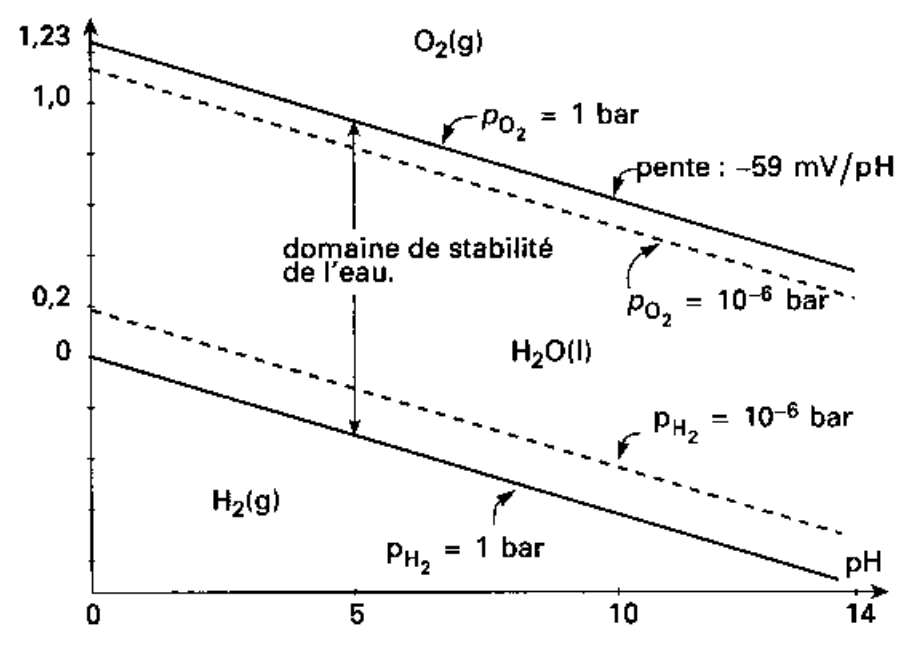
\includegraphics[width=0.54\linewidth]{diagramme_H2O.png}
	\caption{Diagramme E-pH de l'eau pour une pression de tracé de 1\,bar et de $10^{-6}$\,bar. Source : Université de Batna 2.}
\end{figure}

Le diagramme potentiel-pH de l'eau est à connaître par coeur. Il fait intervenir deux couples d'oxydoréduction :
\begin{align}
	&\ce{2 H^+(aq) + 2 e^- = H2(g)} \quad \mathrm{avec} \quad E^\circ(\ce{H^+ / H2}) = 0\,{\rm V} \\
	&\ce{O2(g) +4 H^+(aq) + 4 e^- = 2 H2O(l)} \quad \mathrm{avec} \quad E^\circ(\ce{O2 / H2O}) = 1.23\,{\rm V} 
\end{align}

Ce diagramme est toujours à prendre en compte en solution aqueuse, car l'eau y est toujours présente. Le dioxygène est une espèce présente car elle se dissout naturellement dans l'eau, à moins que le réacteur ne soit protégé de l'atmosphère.

\subsection{Evolution spontanée d'un mélange}

Nous avons vu qu'une réaction est généralement quantitative lorsque le potentiel standard du couple rédox associé à l'oxydant est supérieur au potentiel standard du couple rédox associé au réducteur. Dans ce cas de figure, les domaines de prédominance des deux réactifs sont disjoints, alors que les domaines de prédominance des produits sont superposés. On peut en déduire la propriété générale suivante :
\begin{proposition}
	Deux espèces dont les domaines de prédominance sont disjoints dans un diagramme potentiel-pH vont spontanément réagir pour former des composés dont le domaine est superposé.
\end{proposition}

\section{Corrosion}

Les diagrammes potentiel-pH et le concept de pile nous permettent d'interpréter les phénomènes de corrosion, qui posent problème pour un certain npmbre de dispositifs. 

\subsection{Définition}

\begin{capex}
	En superposant les diagrammes de l'eau et du fer, expliquer ce qui se produit lorsqu'un morceau de fer est exposé à de la pluie ou de l'eau de mer. Que se passe-t-il en milieu acide ? En milieu basique ?
\end{capex}

\begin{definition}
	La corrosion est le phénomène électrochimique par lequel les métaux et alliages subissent de leur environnement une attaque qui les fait évoluer à l'état d'ion métallique par une réaction d'oxydation. Dans le cas où cet environnement est une solution aqueuse, on parle de corrosion humide des métaux.
\end{definition}

\begin{remark}
	On s'accorde, par convention, à utiliser des diagrammes potentiel-pH avec une concentration de tracé de $10^{-6}$\,mol$\cdot$L$^{-1}$ pour étudier les phénomènes de corrosion. En effet, cette concentration d'équilibre dans le solution est jugée suffisante pour mener, sur le long terme, à des dégâts significatifs sur les métaux.
\end{remark}



\subsection{Phénomène de passivation}

On donne le diagramme potentiel-pH de l'aluminium. Lorsqu'il est en contact avec de l'eau, son oxydation mène à la formation de l'oxyde $\ce{Al2O3(s)}$. Ce composé est solide et suffisamment résistant pour protéger l'aluminium de la solution aqueuse. AInsi, une fois qu'une fine couche d'oxyde d'aluminium s'est formée, le métal ne subit plus aucune corrosion :
\begin{definition}
	On parle de passivation lorsqu'un métal subit une oxydation menant à la formation d'une couche superficielle de solide qui vient protéger le métal de la solution. Le métal est alors protégé de la corrosion à long terme.
\end{definition}

\begin{figure}[htbp]
	\centering 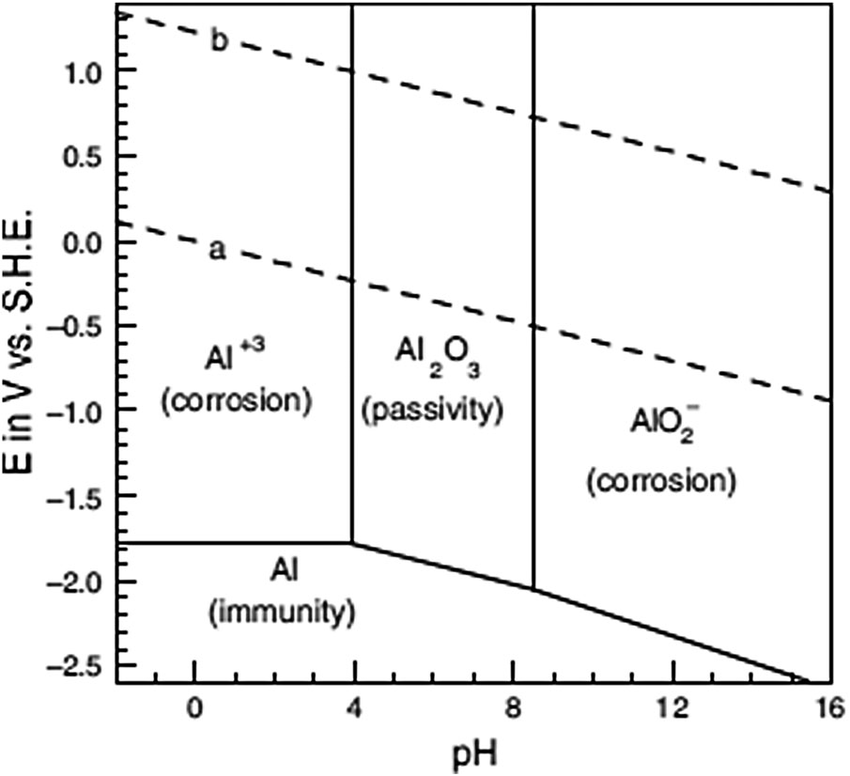
\includegraphics[width=0.45\linewidth]{E_pH_Al.png} 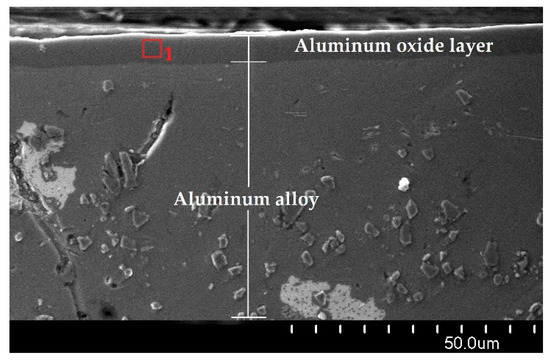
\includegraphics[width=0.54\linewidth]{oxyde_aluminium.jpg}
	\caption{A gauche : diagramme potentiel-pH de l'aluminium, avec les domaines d'immunité, de corrosion et de passivation. A droite : Image d'une couche d'oxyde d'aluminium observée au microscope. Sources : Namitha, K., Rao, P., \& Rao, S. A. (2022). \textit{A brief insight into the use of plant products as green inhibitors for corrosion mitigation of aluminium and aluminium alloys.} Canadian Metallurgical Quarterly, 61(4), 429-441. Niedźwiedź, M., Bara, M., Skoneczny, W., Kaptacz, S., \& Dercz, G. (2022). \textit{Influence of anodizing parameters on tribological properties and wettability of Al2O3 layers produced on the EN AW-5251 aluminum alloy.} Materials, 15(21), 7732.}
\end{figure}

Nous pouvons alors définir trois domaines : le domaine d'immunité, le domaine de corrosion, et le domaine de passivation :
\begin{definition}
	On appelle domaine d’immunité du métal son domaine de stabilité dans le diagramme de corrosion.
Dans cette zone, il est thermodynamiquement stable et ne peut pas être oxydé.

	Le domaine de corrosion est le domaine de stabilité des cations solubles.

	Le domaine de passivation est le domaine de stabilité des oxydes et hydroxydes solides.
\end{definition}


\begin{figure}[p]
	\centering 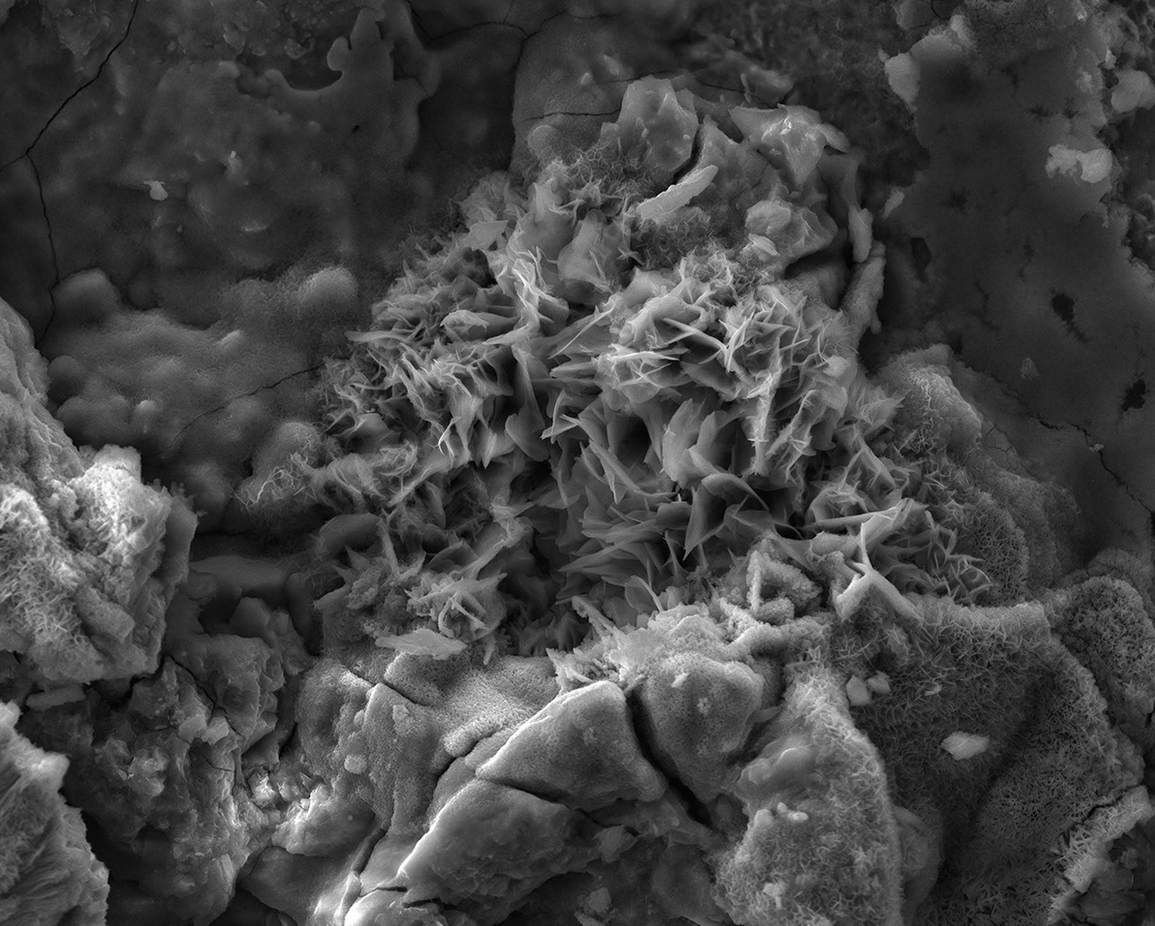
\includegraphics[width=0.85\linewidth]{rouille_microscope_guyane.png} 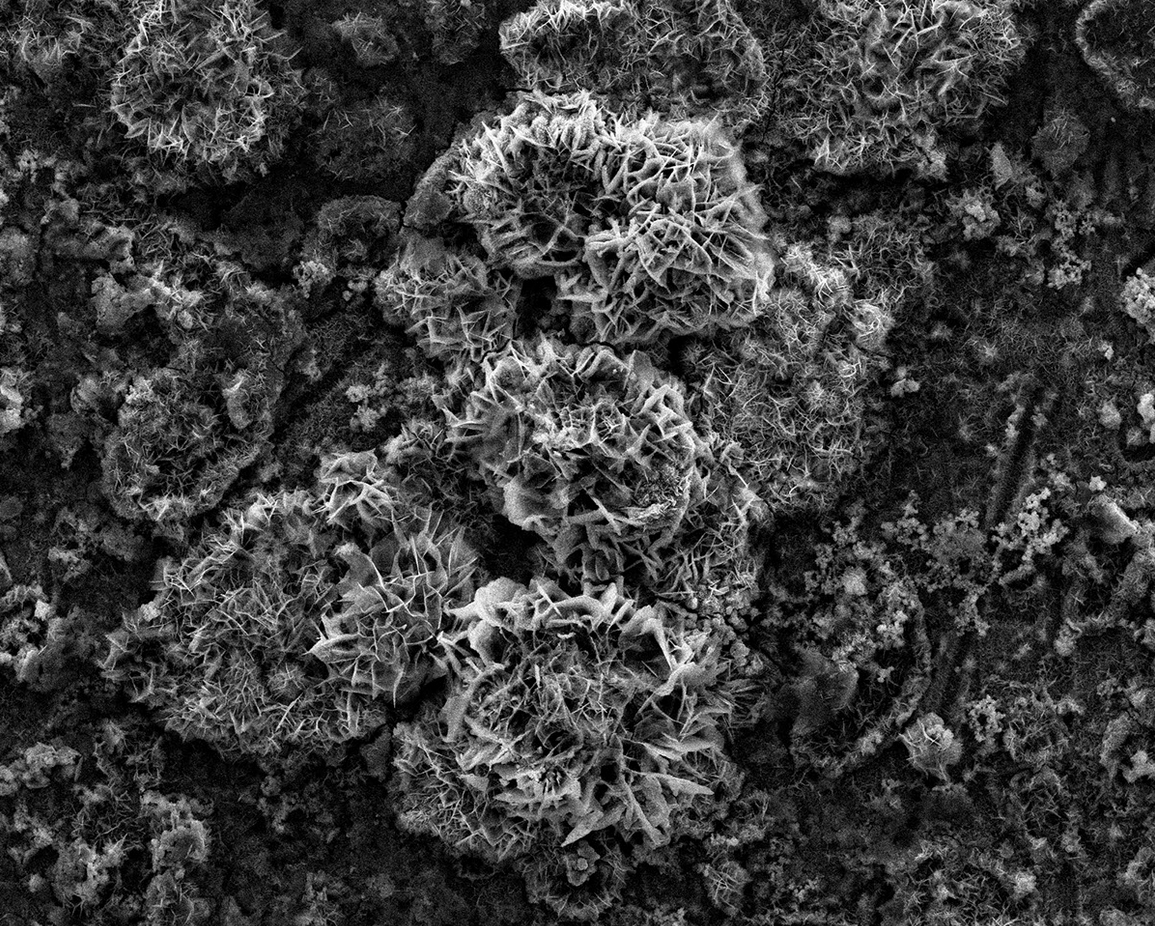
\includegraphics[width=0.85\linewidth]{rouille_guyane_2.png}
	\caption{Images de plaques de fer corrodées par la pluie (en haut, grossissement $\times 3000$) et l'eau de mer (en bas, grossissement $\times 1000$). Source : Laboratoire des Matériaux et molécules en milieu amazonien, Cayenne.}
\end{figure}

\begin{encart}[La rouille en milieu tropical]
	Dans le cas du fer, l'action de l'eau et du dioxygène de l'air conduisent à la formation de la rouille $\ce{Fe(OH)3}$. On pourrait alors penser qu'un phénomène de passivation va protéger le fer, qui ne sera attaqué qu'en surface. Ce n'est pas du tout ce que l'on observe : sans action protectrice, le métal est rapidement entièrement corrodé. Ceci s'explique par la structure microscopique de la rouille, qui est organisé par des microorganismes et forme des structures fractales poreuses à travers lesquelles le dioxygène de l'air et la solution aqueuse peuvent s'infiltrer, permettant à la corrosion de toujours se produire plus en profondeur.
	
	En Guyane, le laboratoire des Matériaux et molécules en milieu amazonien s'intéresse à des méthodes naturelles (notamment à partir de la biodiversité amazonienne) afin de ralentir les phénomènes de corrosion en milieu tropical.	
\end{encart}










\end{document}
